\documentclass[portrait, a0]{a0poster}
%\documentclass[landscape, a0]{a0poster}

\pagestyle{empty}
\setcounter{secnumdepth}{0}

\usepackage[absolute]{textpos}
\usepackage{graphicx}
\usepackage{charter}
\usepackage{palatino}
\usepackage{amssymb,amsmath}
\usepackage{mflogo}
\usepackage{url}

\usepackage{caption}
\captionsetup{font=normalsize, labelfont={color=white,sf,bf}, textfont={color=white,it}}

\usepackage{color}
\definecolor{BurntOrange}{rgb}{1.0,0.3,0.0}
\pagecolor{black}
\TPGrid[40mm,40mm]{26}{12}      % 3 cols of width 8, plus 2 gaps width 1

\parindent=0pt
\parskip=0.5\baselineskip
\def\Heading#1{\noindent{\hfill{\LARGE{\color{BurntOrange} \bf #1}}}\medskip\hrule}
\def\SHeading#1{\medskip\par\noindent{\Large\color{BurntOrange} \it #1}\medskip}
\def\SSHeading#1{\medskip\par\noindent{\large\color{BurntOrange} #1}\medskip}
\begin{document}
%include heading
\begin{figure}
    \centering
	
\includegraphics{pics/Title.png}
    %\VeryHuge{\textcolor{white}{Particle Swarm Frequency Planning}}
\end{figure}

%include names
\begin{textblock}{26}(0,1)
 \begin{center}
   \Large{\textcolor{white}{W. Bezuidenhout, G.B O'Reilly}} \\
   \Large{\textcolor{white}{University of Johannesburg}} \\
 \end{center}
\end{textblock}

%include logo
\begin{textblock}{8}(18,11)
\centering

\includegraphics{pics/ujlogowb.png}
\end{textblock}

%col 1
\begin{textblock}{8}(0,2)
\Heading{Frequency Planning}


\SHeading{Wireless Networks}
\color{white}

In the information age we currently live in almost every device has some sort of wireless technology it uses to provide a specific service. Radios for audio entertainment; Television remotes to change 
channels; Cellular phones for communication; Wireless access points to create wireless LAN's. Wireless technology is now part of our everyday life.

The popularity and rapid adoption of wireless technology hasn't been kind to the management, planning and operation of wireless networks; It has actually worsened a problem known as the Frequency Assignment problem (FAP) which is present in all forms of wireless communication especially in GSM Cellular networks {[1]}.

\SHeading{The Frequency Assignment Problem}

The Frequency Assignment Problem (FAP) is a generalisation of the graph-colouring problem and is subsequently an NP-hard problem{[1]}. This is because one has a finite amount of frequencies which need to be assigned to antennae or tranceivers (TRX's)  where the amount of tranceivers to be assigned frequencies greatly out weigh the amount of available frequencies. Thus it is inevitable that a network will have interference and we can only minimise the amount of interference that might occur on the network - an optimisation problem. 

A contributing factor to the difficulty of the FAP is due to the scarcity of usable frequencies in the radio spectrum, which forces network operators to reuse their allocated / licensed frequencies in their respective networks {[2]}.

The scarcity of the usable frequencies in the spectrum can be attributed to the overuse of certain bands as well as large scale reuse of frequencies in networks. This has put strain on the spectrum and has complicated the management of networks significantly because interference is more likely to occur {[1]}.

\SHeading{Interference}

Interference occurs when frequencies assigned to connections differ by a small margin. The amount of inference on a connection defines the quality of service. 

One can naturally make the deduction that the more frequencies differ used on connections in a area, the better quality of service one will experience in that area. Cellular networks use the amount of interference on their networks as a measure for their \emph{Quality of Service} (QoS) {[2]}.

A network with high interference will experience a lot of dropped connections, which occurs when the interference is too high to sustain a connection for reliable communication.

Primarily interference occurs if the Electromagnetic constraints are violated, which are defined as:
\begin{itemize}
\item \textsl{Co-Channel} -- Two channels are not allowed to have to same allocated frequency
\item \textsl{Adjacent Channel} -- Frequencies assigned to two channels must differ by a certian margin which is usually one
\item \textsl{Co-Cell} -- Any pair of frequencies assigned to a cell must have a certain distance in the frequency domain to prohibit the cell from interfering with other cells on the same site.
\end{itemize}

A fourth constraint called the \emph{Handover} constraint is also applicable in Cellular networks. In Cellular networks handover is the process of transfering your active call from the current cellphone tower that is handling your call to another cellphone tower {[2]}.

Handover is a neccacity in cellular networks since it is the process that ensures that your call isn't dropped while you are moving. With regard to Frequency assignment, the Handover constraint ensures that when a call is transferred that the new allocated frequency for the call differ by a safe margin to minimise interference on the call with other calls that are in progress.

%Let $ T = \{\, t_{2},t_{2},...,t_{n}\,\}$ be a set of \emph{n tranceivers}, and let $ F_{i} = \{\, f_{i1},...,f_{ik}\,\} \subset \mathbb{N}$ be a set of valid \emph{Frequencies} that can be assigned to a transceiver $ t_{i} \in T \mid i \in \{\, 1,2,...,n\,\}$. Futhermore let $ S = \{\,s_{1},s_{2},...,s_{m}\,\} \mid m \in \mathbb{N}$ be a set of \emph{sectors} or \emph{cells}. Each $t_{i} \in T$ is installed at one sector $m$. 

\end{textblock}

%col 2
\begin{textblock}{8}(9,2)
\Heading{Swarm Intelligence}

The Meta Heuristic field has seen an influx of research in recent years due to the success of these algorithms on NP-Complete problems. Swarm Intelligence falls under the Meta Heuristic field. Swarm Intelligence is the notion of entities working together in a group to solve a problem.

Swarm intelligence borrows extensively from research conducted on swarm based life forms like bees, birds, fish and ants. Consequently algorithms that have emerged from these studies are Ant Colony Optimization (ACO) and the Particle Swarm Optimization (PSO).

\SHeading{Particle Swarm Optimization (PSO)}

The standard Particle Swarm Optimization (PSO) algorithm is based on the behavior of birds flying towards a nesting ground or food source. In a flock of birds any individual bird in the flock can influence the behavior and movement of the whole flock.To mimic this behaviour in a algorithm each bird is considered a particle and the food source is considered the global optimum {[3]}.

Each particle (bird) knows its personal best position (personal best cost or optimum) that it has found as well as the globally best position found in the swarm. It uses its personal best and the globally best to adjust its velocity to fly/move towards a better position. With the global sharing taking place in the standard algorithm each particle can benefit from discoveries made by other individual particles.

In the local version of the algorithm each particle does not know the global best found in the swarm rather is only knows the best solution found in its local neighborhood and its personal best position . With the conservative sharing in the local based algorithm, the swarm will not as easily converge to a solution as the global based one. Consequently the local version will search a larger search space. 

\SHeading{Optimization Test Functions}

There are a variety of mathematical functions that test an algorithm with regard to how good it is in finding the global optimum. These formulae are of such a nature that an algorithm can easily get stuck on local minima. Thus they can also be considered as measure of how good an algorithm is in breaking out of local minima. A test function with lots of local minima and only one global minima at $x_{i} = 420.9687, i = 1,...,n$ is the Schwefel function (Figure ~\ref{fig:schwefel}) {[4]}.

% How the Schwefel function was generated with GNUPlot
% set terminal png
% set xrange [-400:400]
% set yrange [-400:400]
% set view 60,30,1,1 (xrotation,zrotation,zoom,zoom)
% set output "schwefel.png"
% splot -x*sin(sqrt(abs(x))) - y*sin(sqrt(abs(y))) with pm3d
\begin{figure}
\centering
\color{black}
\begin{tabular}{c}
\\
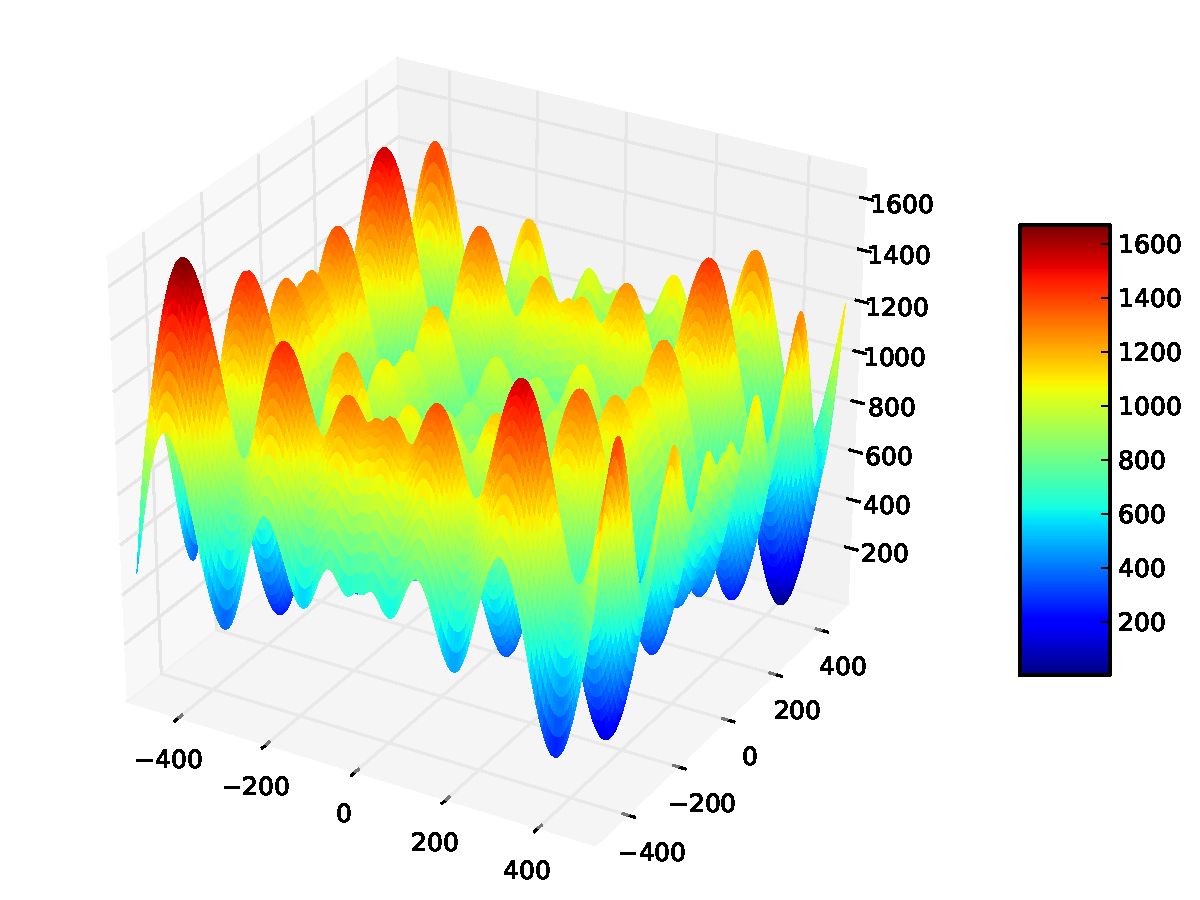
\includegraphics[scale=1.0]{pics/Schwefel.pdf}
\end{tabular}
\color{white}
\caption{The Schwefel Function \label{fig:schwefel}}
\end{figure}
% Insert Camel Hump, Shekels Foxhole, The one that only works with inertia.


\SSHeading{Effect of inertia}

Each object that moves with a certain velocity also has momentum which carries it forward. In the initial PSO algorithm particles only moved based on their velocity. Recent improvements to the PSO algorithm factors the idea of inertia in with the calculation of the particle velocity.

When inertia is included into the calculation it alters how the particles converge to a solution. A high inertia lets the swarm explore aggresively where as a low inertia value lets the swarm converge on a value very quickly. Depening on the search domain one has to different values of inertia to get optimal results.

\end{textblock}

%col 3

\begin{textblock}{8}(18,2)
\begin{figure}
\centering
\begin{tabular}{c}
\\
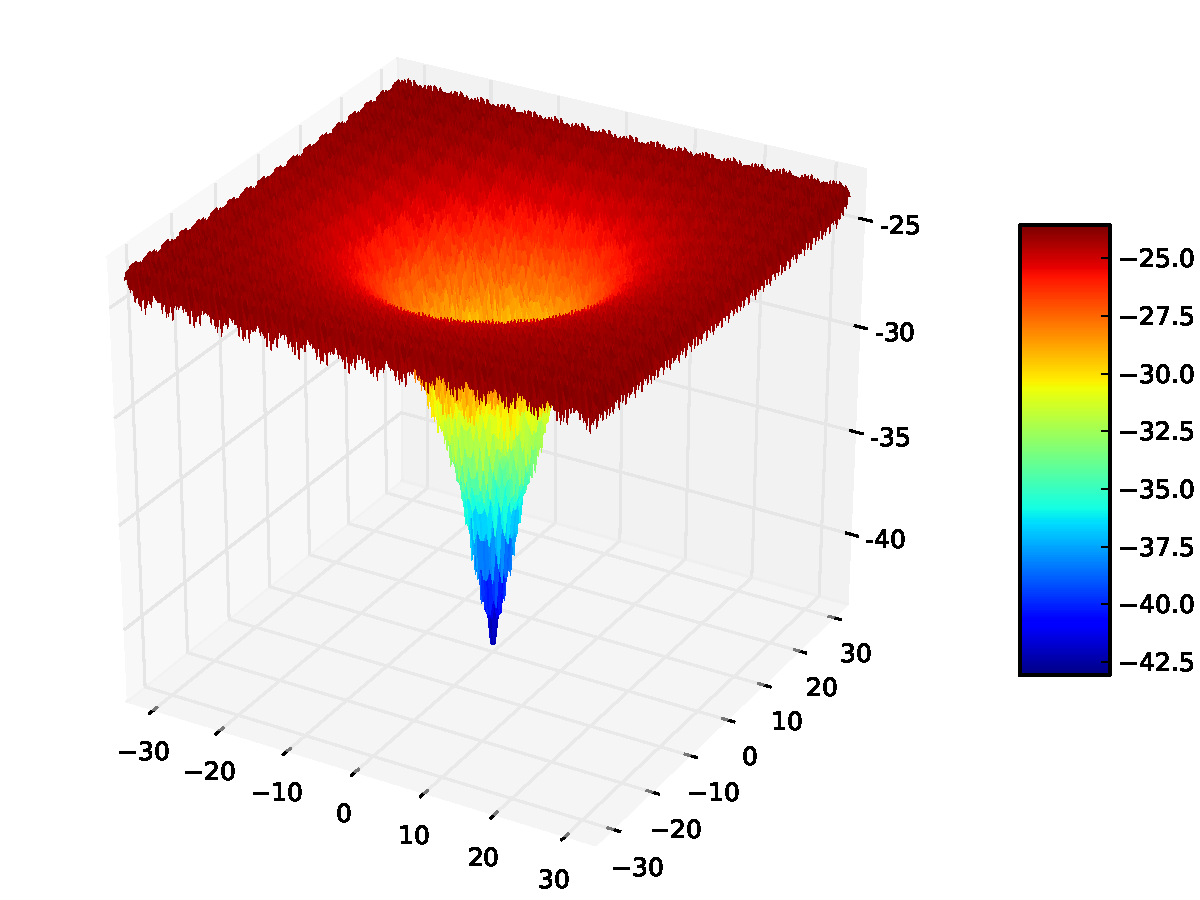
\includegraphics[scale=1.0]{pics/Ackley.pdf}
\end{tabular}
\color{white}
\caption{\textcolor{white}{The Ackley Function \label{fig:DropWaveFunction}}}
\end{figure}

\begin{figure}
\centering
\begin{tabular}{c}
\\
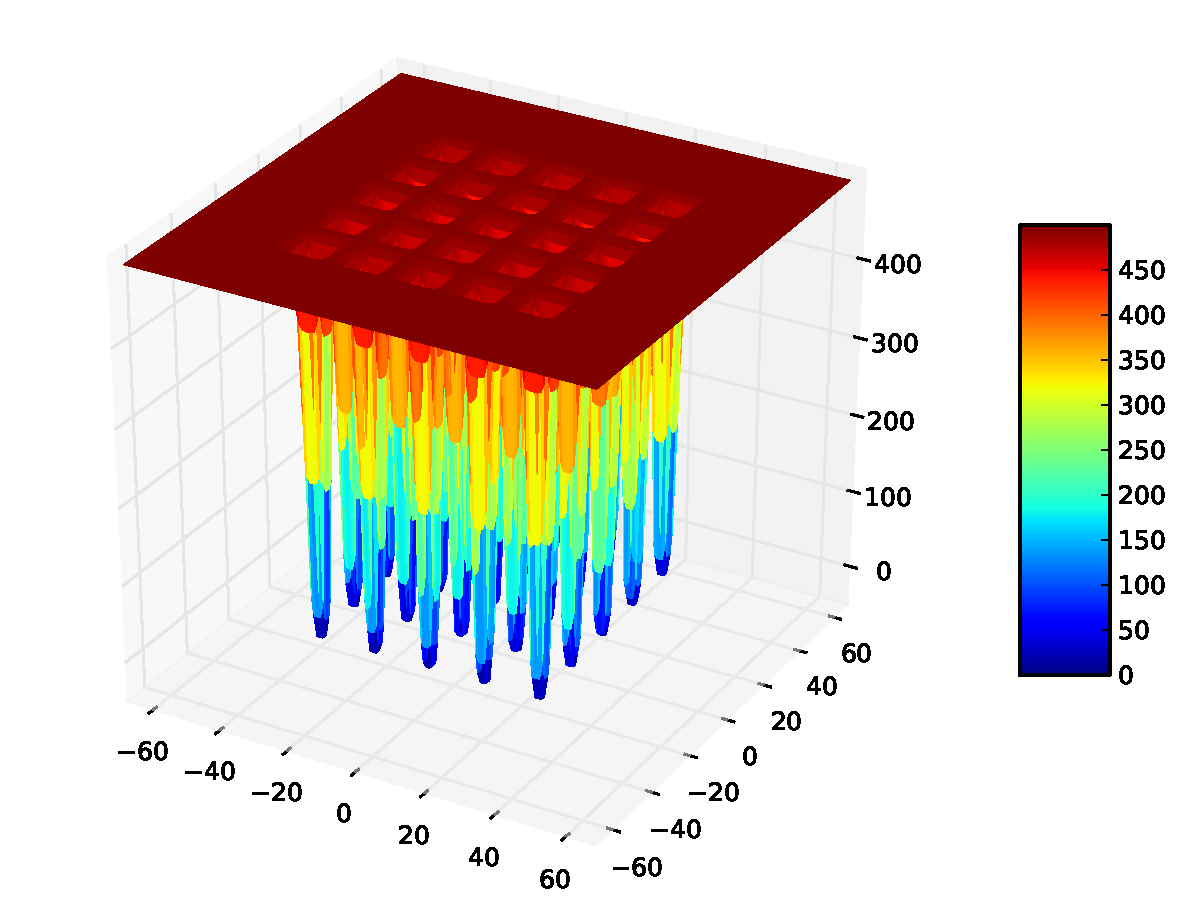
\includegraphics[scale=1.0]{pics/Shekel.pdf}
\end{tabular}
\color{white}
\caption{\textcolor{white}{The Shekel Function\label{fig:logicalmappings}}}
\end{figure}

\Heading{Results}

Before applying the Particle Swarm Optimization algorithm on the Frequency Planning domain, one has to first understand the strength and weaknesses of the algorithm. Thus we, the authors, developed a smallparticle swarm to test on variety of optimization test functions. Below is table depicting the test functions that were used and whether the optimum was found with in 200 iterations.

\begin{center}
\begin{tabular}{| l | c |}
	\hline
	\textbf{Function} & \textbf{Found Optimum} \\
	\hline
	DeJong F1 & Yes \\
	\hline
	Shekel's Foxholes & Yes \\
	\hline
	Rastrigin & Yes \\
	\hline
	Schwefel & No \\
	\hline
	Griewank & Yes \\
	\hline
	Salomon & Yes \\
	\hline
	Six Camel Hump & No \\
	\hline
	Shubert & Yes \\
	\hline
	Himmelblau & No \\
	\hline
	Rosenbrock & Yes \\
	\hline
	Easom & Yes \\
	\hline
	Branins & Yes \\
	\hline
	Michalewicz & No \\
	\hline
\end{tabular}
\end{center}

\SHeading{References}

{[1]} Karen I. Aardal, Stan P. M. van Hoesel, Arie M. C. A. Koster Contact,Information, Carlo Mannino and Antonio Sassano. Models and solution techniques for frequency assignment problems. 4OR: A Quarterly Journal of Operations Research, 1(4):261–317, December 2004.\\
{[2]} Eisenblätter, A., Koster, A. (2007, 01 02). Retrieved 04 03, 2009, from FAP web - A website about Frequency Assignment Problems : http://fap.zib.de\\
{[3]} O'Niel, M., Brabazon, A. (2008). Self-organising swarm (SOSwarm). Soft Computing (12), 1073-1080.\\
{[4]} Marcin Molga, Czesław Smutnicki, Test functions for optimization needs, 3 kwietnia 2005.

\end{textblock}

%footer
\begin{textblock}{8}(0,12)
\footnotesize
Produced using \LaTeXe\ and GNUPlot.
\end{textblock}

\end{document}
